\chapter{Referencial Teórico}


\section{História e Evolução dos Jogos Digitais}

Neste capítulo, exploraremos a história dos jogos eletrônicos e sua evolução ao longo do tempo, com um foco específico no Brasil, estabelecendo uma conexão direta com o tema deste documento.

\subsection{Primeiros Jogos e o Surgimento da Indústria}

O desenvolvimento dos primeiros jogos eletrônicos ocorreu em um cenário muito diferente do atual, quando os próprios criadores precisavam construir seus sistemas do zero, sem \textit{engines} ou ferramentas especializadas. Jogos como \textit{Tennis for Two} (1958) e \textit{Spacewar!} (1962) foram experimentos acadêmicos desenvolvidos em computadores de grande porte, sem qualquer preocupação comercial. A indústria começou a se consolidar na década de 1970, com o lançamento de \textit{Pong} (1972) pela Atari, popularizando o conceito de jogos eletrônicos como uma forma viável de entretenimento \cite{kent2001}.

No Brasil, os jogos eletrônicos chegaram de forma limitada devido ao alto custo de importação. Nos anos 1980 e 1990, surgiram consoles alternativos e um mercado de adaptações.

\subsection{Jogos nos Dias Atuais e Tendências}

Atualmente, a indústria dos jogos digitais está mais acessível, principalmente devido ao surgimento de \textit{engines} como Unity, Unreal Engine e Godot, que permitem que estudantes e desenvolvedores independentes criem jogos sem precisar programar tudo do zero. Esse avanço é particularmente relevante no Brasil, onde o desenvolvimento de jogos ainda enfrenta desafios, como a falta de investimentos e o alto custo de hardware.

Um dos fenômenos mais marcantes da atualidade é o crescimento dos jogos \textit{indie}, desenvolvidos por pequenos estúdios ou até mesmo por indivíduos. Diferente das grandes produções AAA, que exigem orçamentos milionários, os jogos independentes apostam em criatividade, mecânicas inovadoras e narrativas únicas para conquistar o público. Plataformas como a Steam facilitaram a distribuição desses jogos, permitindo que produções de baixo orçamento alcançassem grandes sucessos.

Com essa democratização das ferramentas e do acesso ao conhecimento, o desenvolvimento de jogos digitais se tornou uma oportunidade viável para iniciantes aprenderem na prática. Este trabalho explora esse processo por meio da criação de um jogo do gênero Tron, analisando os desafios e aprendizados envolvidos. A experiência servirá como um estudo de caso para compreender o ciclo de desenvolvimento, aplicando metodologias da engenharia de software e fornecendo um guia para futuros desenvolvedores.

\section{Desenvolvimento de Jogos}

Neste capítulo, abordaremos a parte técnica do trabalho, com foco no desenvolvimento de jogos utilizando práticas de engenharia de software. O objetivo é demonstrar como essas práticas podem contribuir para a criação de jogos eletrônicos, considerando que, assim como qualquer outro produto digital, um jogo também é essencialmente composto por software. Também discutiremos, de forma breve, o funcionamento das \textit{engines} de jogos, ressaltando que, embora o foco do trabalho não seja um estudo aprofundado sobre \textit{engines}, elas desempenham um papel fundamental no processo de desenvolvimento.

\subsection{Engenharia de Software Aplicada a Jogos}

No desenvolvimento de jogos, a Engenharia de Software desempenha um papel fundamental para garantir que o processo seja eficiente, escalável e focado na entrega de um produto de alta qualidade.

\begin{quote}
\small
``Engenharia de software é uma disciplina de engenharia cujo foco está em todos os aspectos da produção de software, desde os estágios iniciais da especificação do sistema até sua manutenção, quando o sistema já está sendo usado.'' \cite{sommerville2011}
\end{quote}

A aplicação de práticas de Engenharia de Software no contexto de desenvolvimento de jogos não se limita à codificação, mas envolve também o gerenciamento de projetos, design e testes.

Conforme Nikhil Malankar discute em seu vídeo, o ciclo de vida de um jogo segue uma estrutura semelhante ao de um software, com etapas de testes e elaboração de requisitos, desde a escolha da plataforma até a implementação final \cite{malankar2023}.

No projeto em questão, as práticas de engenharia de software me ajudaram a organizar, planejar e orientar as etapas de desenvolvimento do jogo. Nas etapas iniciais, mesmo sem iniciar o desenvolvimento, já pude perceber como a aplicação de metodologias como Scrum e MDA pode trazer clareza e eficiência para o processo. Ao seguir essas práticas, o projeto será conduzido de maneira estruturada, com entregas claras e bem definidas em cada ciclo. Além disso, a abordagem de modelagem e os testes iterativos contribuirão para refinar o jogo conforme ele evolui, minimizando erros e ajustando o produto para oferecer a melhor experiência possível.

\subsection{Escolha da Engine para o Jogo}

Para desenvolver um jogo, é essencial definir as necessidades técnicas. As \textit{engines}, ou motores de jogos, desempenham um papel central nesse processo. Uma \textit{engine} é um software que integra um conjunto de ferramentas e recursos projetados para simplificar e otimizar o desenvolvimento de jogos, abrangendo elementos como gráficos, física, som e muito mais. Além de acelerar o processo de produção, o uso de uma \textit{engine} garante maior eficiência e qualidade no resultado final \cite{pixstudios}.

Embora seja possível criar uma \textit{engine} própria, essa abordagem geralmente é recomendada apenas em casos específicos, como atender a requisitos altamente personalizados ou aprofundar o entendimento técnico do desenvolvimento de jogos. No entanto, construir uma \textit{engine} do zero é uma tarefa complexa e demorada, exigindo meses de trabalho para implementar funcionalidades básicas, como renderização gráfica e gerenciamento de recursos, antes mesmo de iniciar o desenvolvimento do jogo em si. Por outro lado, \textit{engines} amplamente utilizadas, como Unity, Unreal Engine e Godot, já oferecem essas funcionalidades de maneira robusta e otimizada. Além disso, elas contam com suporte técnico, documentação abrangente e comunidades ativas, permitindo que o desenvolvedor concentre seus esforços na criação e no design do jogo, sem a necessidade de reinventar ferramentas fundamentais \cite{ullmann2022}.

Para garantir a escolha mais adequada da \textit{engine} para este projeto, foi realizado um estudo comparativo entre duas opções amplamente reconhecidas: Unity e Godot. Cada uma foi avaliada com base em critérios específicos, como:

\begin{itemize}
    \item Facilidade de aprendizagem e qualidade da documentação;
    \item Suporte a múltiplas plataformas;
    \item Licenciamento e custos;
    \item Linguagem de programação utilizada;
    \item Recursos e ferramentas disponíveis;
    \item Adequação ao tipo de jogo a ser desenvolvido.
\end{itemize}

Este estudo forneceu uma base sólida para a escolha da \textit{engine} mais alinhada às necessidades e objetivos do projeto.

\subsubsection{Comparação entre Game Engines (Godot vs Unity)}

O desenvolvimento de jogos exige a escolha de uma \textit{engine} que atenda às necessidades do projeto. Neste comparativo, analisamos Unity 6 e Godot 4 como principais alternativas, considerando fatores como facilidade de uso, desempenho em jogos 2D, custos e requisitos técnicos. Como o objetivo deste trabalho é apresentar um guia e desenvolver um jogo de baixo custo, a escolha deve priorizar acessibilidade e eficiência \cite{godot-sysreq} \cite{unity-sysreq}.

\begin{table}[H]
\centering
\caption{Análise comparativa geral entre engines}
\label{tab:comparacao-engines}
\begin{tabularx}{\textwidth}{|>{\bfseries}l|X|X|}
\hline
\textbf{Critério} & \textbf{Unity 6} & \textbf{Godot 4} \\
\hline
Facilidade de Uso & 
Interface robusta com muitas funcionalidades, mas complexa para iniciantes. Utiliza C\# como principal linguagem de programação. & 
Interface leve e simplificada, curva de aprendizado menos íngreme. Oferece GDScript, semelhante ao Python, facilitando o desenvolvimento. \\
\hline
Desempenho em Jogos 2D & 
Suporte a 2D, mas originalmente projetado para 3D. Recursos são adaptados do ambiente 3D, podendo resultar em menos eficiência. & 
Motor 2D do Godot, apesar de funcionar tanto para 3D como 2D, o motor 2D é considerado um aspecto forte da engine. \\
\hline
Custo e Licenciamento & 
O uso é gratuito, mas após o lançamento, o modelo de licenciamento pode incluir taxas baseadas no número de downloads. & 
Open-source e totalmente gratuito, sem taxas ou restrições comerciais. \\
\hline
\end{tabularx}

\smallskip
\raggedleft \textbf{Fonte:} Autoria própria.
\end{table}

\begin{table}[H]
\centering
\caption{Comparativo técnico baseado em requisitos}
\label{tab:comparativo-tecnico-engines}
\begin{tabularx}{\textwidth}{|>{\raggedright\arraybackslash}X|>{\raggedright\arraybackslash}X|>{\raggedright\arraybackslash}X|}
\hline
\textbf{Requisitos Técnicos} & \textbf{Unity 6} & \textbf{Godot} \\
\hline
CPU & 
X64 com suporte a SSE2 ou ARM64. Exemplo: Intel Core 2 Duo E8200, AMD Athlon XE BE-2300. & 
X86\_32 com SSE2, X86\_64 ou ARMv8. Exemplo: Intel Core 2 Duo E8200, Raspberry Pi 4. \\
\hline
GPU & 
DX10, DX11, DX12 ou Vulkan-capaz. Exemplo: Intel HD Graphics 5500, AMD Radeon R5. & 
Vulkan 1.0 ou OpenGL 3.3. Exemplo: Intel HD Graphics 2500, AMD Radeon R5. \\
\hline
RAM & 
Mínimo de 8GB, recomendado 16GB ou mais para projetos complexos. & 
Nativo: 4GB; Web editor: 8GB. \\
\hline
Armazenamento & 
Ocupa mais espaço em disco, especialmente com projetos grandes. & 
200MB para execução; exportação requer 1.3GB. \\
\hline
Sistema Operacional & 
Windows 10 21H1+, macOS 11+ (Big Sur), Ubuntu 22.04+ & 
Windows 7+, macOS 10.13+, Linux pós-2016, Web Editor compatível com navegadores modernos. \\
\hline
\end{tabularx}

\smallskip
\raggedleft \textbf{Fonte:} Elaboração própria.
\end{table}

\subsubsection{Análise e critérios para escolha da engine}

Após a análise comparativa entre as duas engines, Godot foi escolhida como a engine mais adequada para o desenvolvimento deste jogo. A decisão foi fundamentada em vários critérios técnicos e de projeto, conforme detalhado abaixo:

\textbf{Facilidade de uso e curva de aprendizagem}
A simplicidade da interface do Godot e a utilização do GDScript, que é uma linguagem de programação semelhante ao Python, tornam o desenvolvimento mais acessível, especialmente para quem está começando ou tem um foco maior na parte lógica do jogo. Isso permite uma curva de aprendizado mais suave, o que é um ponto crucial dado o prazo do projeto e a necessidade de uma implementação eficiente.

\textbf{Desempenho em Jogos 2D}
Embora o Unity ofereça suporte robusto para jogos 2D, a Godot foi projetada desde o início com um motor 2D altamente otimizado. Isso garante que o desempenho da engine em jogos bidimensionais seja superior, além de permitir um maior controle sobre o comportamento do jogo, o que é essencial para um projeto que visa ser leve e de baixo custo, como o proposto.

\textbf{Custo e Licenciamento}
Godot é open-source e totalmente gratuita, sem custos adicionais ou limitações comerciais, o que representa uma vantagem significativa para o projeto. Não há taxas de licenciamento, e o código-fonte da engine pode ser modificado conforme as necessidades específicas do desenvolvimento. Esse fator elimina preocupações com custos futuros e garante flexibilidade total, além de facilitar a utilização sem complicações de licenciamento.

\textbf{Requisitos Técnicos}
A Godot exige menos recursos de hardware, o que torna o desenvolvimento mais ágil, especialmente em termos de tempo e capacidade de testes. Com um espaço de armazenamento inicial de apenas 200MB e suporte para uma ampla gama de sistemas operacionais, como Windows, macOS e Linux, a engine se adequa bem aos requisitos de recursos do projeto e possibilita um desenvolvimento mais fluido, sem depender de máquinas muito potentes.

\textbf{Adequação ao tipo de jogo}
Como o projeto é voltado para a criação de um jogo 2D com mecânicas simples de movimento e interação, a Godot oferece ferramentas e funcionalidades que atendem perfeitamente às necessidades do jogo. O motor 2D da Godot é mais direto e flexível para o tipo de mecânica que estamos desenvolvendo, sem a necessidade de adaptações que seriam necessárias em outras engines.

Por todas essas razões, a Godot se mostrou a escolha mais adequada para este projeto, considerando tanto o orçamento, a complexidade técnica e a necessidade de uma engine eficiente para o desenvolvimento de jogos 2D de baixo custo.


\subsubsection{Conhecendo a Engine Godot}

Como já foi mencionado anteriormente, desenvolver sua própria engine de jogos é uma tarefa desafiadora e envolvente. Porém, para entender como a engine Godot funciona, é interessante compreender quais as funcionalidades mínimas de uma engine de jogos.

Para desenvolver uma engine de jogo, é necessário implementar alguns sistemas essenciais. Esses sistemas são:

\begin{itemize}
  \item \textbf{Inicialização do Sistema}: Basicamente, é abrir uma janela, obter o contexto gráfico (OpenGL/DirectX/Vulkan) e inicializar o áudio.
  \item \textbf{Controle de Tempo ou Game Loop}: Todo jogo precisa ter um loop para controlar a taxa de atualização e renderização do jogo.
  \item \textbf{Entrada de Dados}: Implementar a captura de entradas (botões pressionados).
  \item \textbf{Renderização}: Utilizar computação gráfica para renderizar as texturas na tela.
  \item \textbf{Utilitários Matemáticos}: Bibliotecas de matemática (vetores e matrizes) e funções úteis para o desenvolvimento.
  \item \textbf{Gestão de Objetos e Cenas}: Sistema para gerenciar objetos e cenas à medida que seu jogo se torna mais complexo.
  \item \textbf{Áudio}: Suporte para tocar músicas e efeitos sonoros.
  \item \textbf{Carregamento de Arquivos}: Utilizar um gerenciador de arquivos para evitar o carregamento redundante e permitir a adição de recursos como mods.
\end{itemize}

Tudo isso é apenas o básico, e cada sistema pode variar muito em nível de complexidade \citeonline{glaiel2021}.

\begin{figure}[htbp]
    \centering
    \caption{Game Loop, Sprite e Music}
    \label{fig:GSM}
    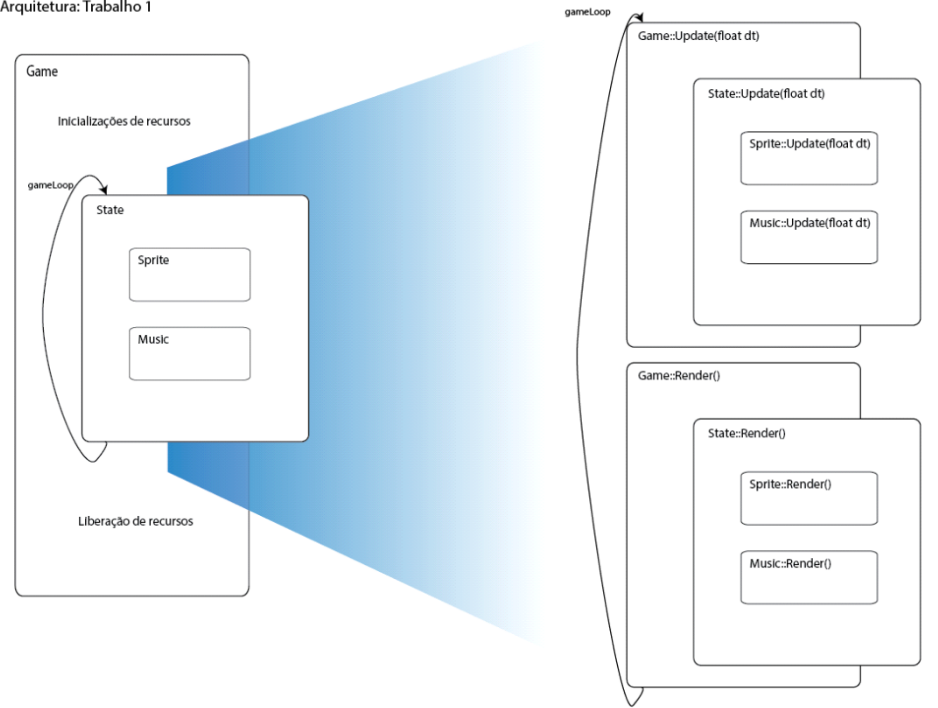
\includegraphics[width=0.7\textwidth]{figuras/cic-engine.png}
    \legend{Fonte: Trabalho 2 - Introdução de Desenvolvimento de Jogo - Departamento de Ciência da Computação UnB.}
\end{figure}

Agora, vamos entender como o Godot traduz tudo isso para dentro de sua engine.

\paragraph{Nodes}

No Godot, \textit{nodes} (ou nós) são os elementos fundamentais que compõem qualquer cena. Existem dezenas de tipos de \textit{nodes}, cada um com uma função específica, como representar objetos gráficos, controlar física, lidar com entradas de usuário ou até organizar o layout de outros nós. Eles são como os sistemas mencionados anteriormente.

\begin{flushright}
\textit{“Nodes are the fundamental building blocks of your game. They are like the ingredients in a recipe. There are dozens of kinds that can display an image, play a sound, represent a camera, and much more.”}
(GODOT ENGINE 4.3 documentation in English, s.d., p. 1)
\end{flushright}

\paragraph{Scenes}

As cenas são as telas que contêm os \textit{Nodes}. Para entender melhor as cenas podemos exemplificar de duas maneiras: através de menus/telas ou \textit{chunks}. No caso do jogo que estamos desenvolvendo, cada cena é representada por uma tela. Já em jogos com grandes mundos, onde a câmera segue o jogador, as cenas podem ser \textit{chunks} e apenas os \textit{chunks} necessários são carregados para gerar a cena. 

Quem controla os recursos para gerar as cenas são os scripts do programador (de forma manual) ou, de forma dinâmica, usando \textit{TileSet}, \textit{TileMap} e recursos de \textit{Resource Management}.

\begin{figure}[htbp]
    \centering
    \caption{Tile Set, Tile Map e Resource Management}
    \label{fig:tiles}
    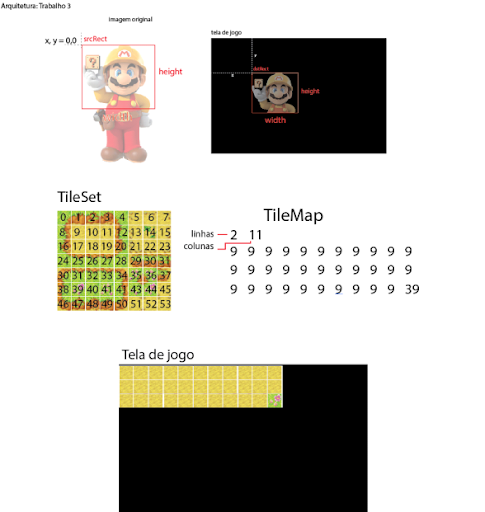
\includegraphics[width=0.7\textwidth]{figuras/tile-map-cic.png}
    \legend{Fonte: Trabalho 3 - Introdução de Desenvolvimento de Jogo - Departamento de Ciência da Computação UnB.}
\end{figure}